\chapter{Wahrnehmung \& Kommunikation}

Jede Interaktion mit der Welt setzt voraus, dass wir die Welt überhaupt wahrnehmen. Das Experiment \textit{Blinder Fleck} zeigt, dass wir die Welt offenbar falsch wahrnehmen.

Unsere Sensoren nehmen Reize wahr und gehen mittels Neuronen übers Rückenmark ans Gehirn. Die Körpergrenze ist das Interface. Siehe dazu auch das Bild in Kapitel Selbstführung \ref{fig:neurale-informationverarbeitung}. Alle Informationen gelangen ins UB, nur ein Teil davon ins Bewusstsein. Geruchs- und Geschmacksinfos können wir nicht filtern. Aktuelle Infos werden mit vorhanden Infos (Gedächtnis) gemischt.

\section{Vom Sehen zum Bild}
\begin{enumerate}
	\item Elementarformen identifizieren. Wir nehmen zuerst folgendes wahr: Kante, Form, Farbe, Flächen, Bewegungen, Gesichter ...
	\item Anschliessend verdichten wir zu Gebilden, wie: Gebäude, Orte, Geräte, Objekte ...
	\item Mustererkennung. Wir assoziieren das Objekt mit Erinnerungen.
\end{enumerate}

\paragraph{Zeitliche Koordination:}
Übertragung der sensorischen Impulse dauert unterschiedlich lange (Fuss-Gehirn, Auge-Gehirn). Für Verarbeitung der Information benötigt das Gehirn unterschiedlich viel Prozessorzeit (Formen/Farben/Texte etc.). Um alles zu einem Gesamtbild zusammenzusetzen, muss es auf den langsamsten Prozess warten. Alle Reize innert 100ms ... 120ms betrachtet das Gehirn als zusammengehörend. 

\paragraph{Wahrnehmung geschieht unbewusst:}
Der grösste Teil der Wahrnehmung geschieht unbewusst und kann vom Bewusstsein nicht beeinflusst werden. Was dem Bewusstsein als Wahrnehmung präsentiert wird, ist eine vom UB aufgebaute, scheinbare plausible Story. Auf die Story haben Erwartungen, Hoffnungen, Erinnerungen genauso starken Einfluss wie die effektiven Umweltreize.

Merksatz: ''Wir glauben, was wir sehen, weil wir sehen, was wir glauben''

\paragraph{Evolution:} [MEP] Die Wahrnehmung hat sich über die gesamte Zeitspanne der Evolution entwickelt. Evolution ist in jedem von uns drin. Jeder Mensch durchläuft abgekürzt die gesamte menschliche Evolution. Auch das Gehirn hat sich entwickelt, die einzelnen Gehirnteile sind übereinander gewachsen:

\begin{description}
	\item[Stammhirn:] aka Krokodil. Schon bei Reptilien \& Vögeln und steuert automatische Reflexe und Körperfunktionen.
	\item[Limbisches System:] aka Pferd aka Zwischenhirn. Frühe Säugetiere und ist für Gefühle und unbewusste Reaktionen verantwortlich.
	\item[Neocortex:] aka Delphin aka Grosshirn. Höhere Säugetiere, Primaten dient für rationales Denken, Vernunft und bewusste Entscheidungen.
	\item[Präfrontaler Cortex:] aka Guru aka Stirnhirn. Menschen, ab ~16j und ist für Mathematik, Kreativität, Meditation etc. da.
\end{description}

Unser Gedächtnis beginnt nicht leer. In jedem von uns sind die nützlichen Erfahrungen unserer Vorfahren bereits verankert. Die jüngsten Erfahrungen (ca. vor 8000 Jahren), Ackerbau und Viehzucht sind bereits zu einem klein Teil körperlich verankert. Das individuelle Gedächtnis ergänzt lediglich eine enorme Menge bereits vorhandener Erinnerungen.

\paragraph{No database:}
Achtung - Das Gedächtnis ist keine Datenbank. Wir speichern nur Bruchstücke. Bei jedem Lese Zugriff auf eine Erinnerungen, nehmen wir diese, und speichern sie meist modifiziert wieder ab. Die Erinnerungen ist ein unzuverlässiges Konstrukt. Tipp von Ernst: Dann modifiziere Sie doch einfach in die bessere Richtung.

\section{Fazit}
Was sich uns als Realität darstellt ist ein vom Unterbewusstsein aus neu eingehenden Informationen, Erinnerungen, Erfindungen und Streichungen
zusammengemischtes, ~100 mS altes Konstrukt.
\begin{itemize}
	\item Wir sehen die Realität, die wir sehen wollen
	\item Was wir sehen wollen, hängt ab von unseren früheren Erlebnissen, aktuellen Erwarutngen und unseren tiefliegenden Glaubensätzen.
	\item Die Konstruktion der Realität erfolgt unbewusst.
\end{itemize}

[MEP] In der Abbildung \ref{fig:wahrnehmung-ablauf} sehen wir den Ablauf der Wahrnehmung.

\begin{figure}[h!]
\centering
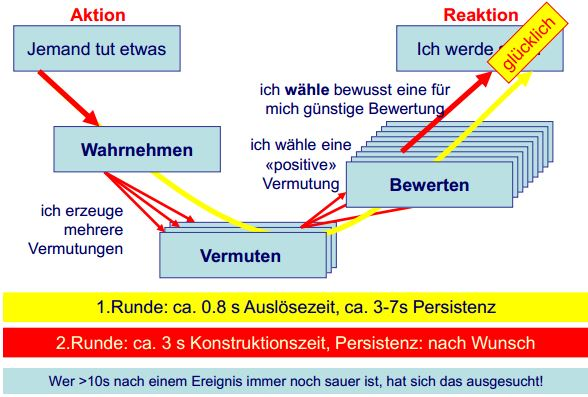
\includegraphics[width=0.7\linewidth]{fig/wahrnehmung-ablauf}
\caption{Wahrnehmungs-Ablauf}
\label{fig:wahrnehmung-ablauf}
\end{figure}

Wahr ist was ich zur Wahrheit bestimme. Gefühle basieren auf MEINER Realität.

\section{What we have learned}
Ich nehme die «Welt da draussen» nicht so wahr, wie sie ist, sondern wie sie mein Unterbewusstsein mir darstellt. Was ich bewusst wahrnehme, ist eine Mischung aus externer Realität, meinem Gedächtnis und meiner
Aufmerksamkeit. Mein Gedächtnis umfasst evolutionäre Erinnerungen und
eigene Lebenserfahrungen – gemischt mit vielem Anderen. Meine Gefühle und Reaktionen werden von meiner Wahrnehmung gesteuert: W-V-B => so fühle ich mich. Ich kann meine spontane Reaktion nicht verhindern, aber dann meine Gefühle selber steuern.

\section{INTEGRO}
Integro ist ein einfaches und praxiserprobtes Modell, um eine wichtige Dimension der Persönlichkeit zu verstehen: Stärken/Schwächen der Wahrnehmung und Eigenheiten der Kommunikation. Dies bezieht sich auf eigene sowie anderer Leute.

\paragraph{Hintergrund:} Menschen sind vielfältig und mehrdimensional, dies macht es schwierig sie zu verstehen. Ein vereinfachtes Modell hilft! Mit der Rückmeldung Anderer bekommt jeder ein klares Bild wie er auf andere wirkt. Wertungsfrei: Das Integro-Modell kennt keine guten oder schlechten Stile. Alle Stile haben ihre Stärken und Schwächen.

\begin{figure}[h!]
\centering
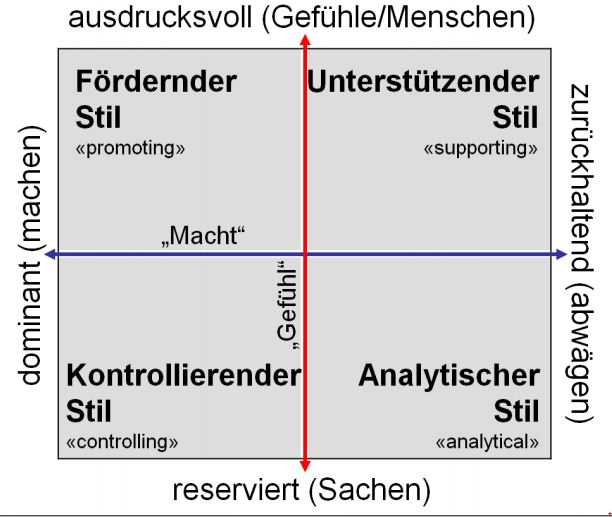
\includegraphics[width=0.5\linewidth]{fig/integro-modell}
\caption{Integro Modell [MEP]}
\label{fig:integro-modell}
\end{figure}

\begin{figure}[h!]
\centering
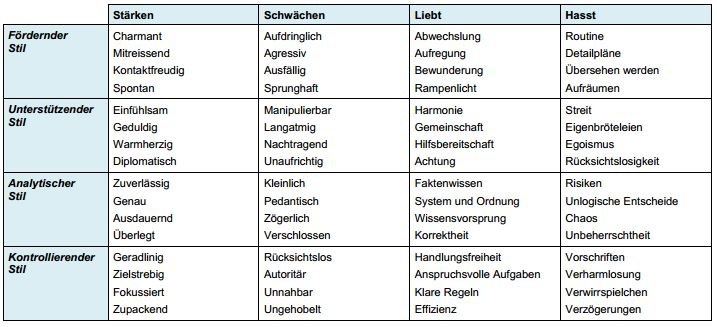
\includegraphics[width=0.7\linewidth]{fig/integro-uebersicht-stile-attribute}
\caption{Integro Übersicht Stile}
\label{fig:integro-uebersicht-stile-attribute}
\end{figure}

\subsection{Flexibilität}
Der eigene Stil ist langfristig stabil. Je nach Situation kann man auch andere Verhaltensweisen zeigen, wie leicht das gelingt zeigt die Flexibilität. Die Flexibiltät umfasst folgende Aspekte:
\begin{itemize}
	 \item die mittlere, allgemeine Neigung zu Flex- oder Inflexibilität
	 \item die momentane Flexibilität in der aktuellen Situation
	 \item die Leichtigkeit, vom stiltypischen Verhalten abzuweichen
	 \item die Reaktion auf Veränderungen und Überraschungen
\end{itemize}
Flexibilität kann man steuern und trainieren. Höhere Flex ist oft erwünscht.